\documentclass[a4paper,12pt]{article}
\setlength\textwidth{7in}
\usepackage[T1]{fontenc}
\usepackage[utf8]{inputenc}
\usepackage{amssymb,amsmath}
\usepackage{verbatim,graphicx}
\usepackage{fullpage}
\usepackage{booktabs,array,longtable,multirow}
\usepackage{url}
\usepackage{hyperref}
\usepackage{enumitem}
\usepackage{float}
\usepackage{placeins}
\usepackage{adjustbox}
\usepackage{tabularx}
\usepackage{xcolor}
\usepackage{tikz}
\usepackage{pgfplots}
\usepackage{caption}
\usepackage{ifthen}
\usetikzlibrary{arrows.meta,positioning,shapes.geometric,shapes.misc,fit}
\pgfplotsset{compat=1.18}
\hypersetup{
    colorlinks=true,
    linkcolor=blue,
    urlcolor=blue,
    citecolor=blue
}
\raggedbottom

\tikzstyle{process} = [rectangle, rounded corners, draw=black, thick, minimum width=3.2cm, minimum height=0.9cm, align=center, fill=blue!8]
\tikzstyle{decision} = [diamond, aspect=2, draw=black, thick, align=center, fill=yellow!15, inner sep=1pt]
\tikzstyle{store} = [cylinder, shape border rotate=90, aspect=0.25, draw=black, thick, minimum height=1cm, minimum width=1.8cm, align=center, fill=green!10]
\tikzstyle{arrow} = [-{Latex[length=3mm]}, thick]
\tikzstyle{cloudbox} = [rectangle, draw=black, thick, rounded corners, fill=gray!8, minimum width=3cm, minimum height=1cm, align=center]
\newcolumntype{Y}{>{\raggedright\arraybackslash}X}

\begin{document}

\begin{titlepage}
\vspace*{1.3cm}
    \begin{center}
    \large{\textbf{Fraud and Abnormal Order Detection in Supply Chain ERP Transactions Using Machine Learning}}
    \end{center}
    \vspace{0.5cm}
    \begin{center}
    \small{\textit{Project progress report submitted} \\ \vspace{0.25cm} \textit{to} \\ \vspace{0.25cm}\textbf{MANIPAL ACADEMY OF HIGHER EDUCATION}}
    \end{center}
    \vspace{0.25cm}
    \begin{center}
    \small{\textit{For Partial Fulfillment of the Requirement for the\\ \vspace{0.25cm}Award of the Degree\\ \vspace{0.25cm}of}} \\ \vspace{0.25cm}
    \textbf{Bachelor of Technology} \\  \vspace{0.25cm} \textit{in} \\ \textbf{Information Technology}
    \end{center}

    \begin{center}
    \small{\textit{by}} \\
    \textbf{Varad Dharmadhikari} \\ \textbf{Reg. No. 190911xxx} \\
    \end{center}

\begin{center}
    \small{\textit{Under the guidance of}} \\
\renewcommand{\baselinestretch}{1}
{
\begin{table}[h]
    \centering
        \begin{tabular}{p{3in} p{3in}}
            Ms.~Ramyashree &  Dr.~ABC (External Guide)  \\
            Internal Guide & External Guide \\
            Department of I \& CT  &  Project Group/Department  \\
             Manipal Institute of Technology & Company/Organization \\
            Manipal, India & Company Address
        \end{tabular}
\end{table}
}
\end{center}

    \begin{figure}[h]
    \begin{center}
    \IfFileExists{MITLogo.png}{
        \includegraphics[width=3cm]{MITLogo.png}
    }{
        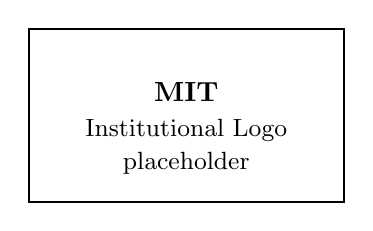
\begin{tikzpicture}
            \draw[thick] (0,0) rectangle (4,2.2);
            \node at (2,1.4) {\textbf{MIT}};
            \node[align=center] at (2,0.7) {\small Institutional Logo\\\small placeholder};
        \end{tikzpicture}
    }
    \end{center}
    \end{figure}
    \begin{center}
    \textbf{April 2026}
    \end{center}
\end{titlepage}

\pagenumbering{roman}
\tableofcontents
\newpage
\listoffigures
\newpage
\listoftables
\newpage

\pagenumbering{arabic}

\section{Introduction}
Fraud and abnormal order behavior in enterprise resource planning (ERP) systems has become a serious operational and financial concern for manufacturing, retail, logistics, and distribution organizations. Modern supply chains process thousands of transactions involving order placement, discount approval, refunds, shipping changes, manual overrides, and returns. Although most transactions are legitimate, a small subset can signal suspicious or fraudulent behavior such as inflated refunds, shipping and billing mismatches, unusual discount patterns, high-value orders from new accounts, and repeated returns linked to prior customer activity.

Traditional manual auditing is not well suited to such data volumes. Manual review is slow, expensive, and inconsistent across teams. This motivates the use of machine learning methods that can score transactions automatically and help investigators prioritize the most suspicious cases. At the same time, practical deployment matters: an academically strong model is not enough if the system cannot accept real inputs, expose results through a usable interface, and persist outputs in a secure cloud environment.

This project addresses that need by developing a complete fraud detection pipeline for ERP-style supply chain transactions. The implemented system accepts uploaded CSV order data, applies preprocessing and validation, generates interpretable fraud-related features, uses a trained Random Forest model to compute a fraud risk score, and returns a suspicious flag for each record. The system has been designed to operate in two modes:
\begin{itemize}[noitemsep]
    \item \textbf{Local machine mode}, where the frontend and backend run on localhost for experimentation, training, and demonstration.
    \item \textbf{Azure-enabled mode}, where the backend can be hosted online and store generated outputs in Azure Blob Storage.
\end{itemize}

The overall research contribution lies in combining explainable fraud analytics with a lightweight deployment architecture that is suitable for a final-year B.Tech project, yet technically aligned with real-world cloud deployment practices. The work also highlights an important observation from the broader fraud detection literature: high classification performance alone is not sufficient. Robust preprocessing, careful handling of imbalanced data, interpretable feature design, and reliable deployment are equally important for operational usefulness \cite{abdallah2016survey,sorournejad2016survey,ahmed2016anomaly,sulaiman2022review}.

\section{Literature Survey}
Fraud detection has been extensively studied in domains such as banking, e-commerce, insurance, and cybersecurity. However, supply chain and ERP-style transaction fraud remains comparatively less explored, especially in the context of deployable student-friendly systems. This section summarizes the most relevant literature and positions the present work within that research landscape.

Abdallah \textit{et al.} \cite{abdallah2016survey} provide a foundational survey of fraud detection systems and identify common challenges such as concept drift, class imbalance, delayed labels, and the need for real-time or near-real-time decisions. Their work is especially useful for understanding why fraud detection differs from ordinary classification problems.

Sorournejad \textit{et al.} \cite{sorournejad2016survey} present a data- and technique-oriented survey of credit card fraud detection methods. They compare supervised, unsupervised, and hybrid techniques and emphasize the importance of preprocessing and feature construction. While their domain is financial card data, the methodological lessons transfer well to ERP transaction settings.

Ahmed \textit{et al.} \cite{ahmed2016anomaly} review anomaly detection techniques in the financial domain and show how outlier-based reasoning complements supervised classification. Their survey highlights that unsupervised methods can be useful when labeled fraud examples are scarce, but they can also produce less interpretable alerts and require careful threshold selection.

Sulaiman \textit{et al.} \cite{sulaiman2022review} analyze modern machine learning approaches for fraud detection and discuss privacy-preserving directions such as federated learning. Their review shows that Random Forest, support vector machines, and neural approaches each offer benefits, but model choice must be balanced against interpretability, dataset availability, and deployment complexity.

Afriyie \textit{et al.} \cite{afriyie2023supervised} report strong results for supervised learning algorithms in fraud detection and observe that ensemble classifiers often outperform simpler baselines. Their work supports the use of tree-based models as strong starting points for structured tabular data.

Lin and Jiang \cite{lin2021autoencoder} propose a hybrid Autoencoder and Probabilistic Random Forest method that improves modeling of complex fraud patterns. Although powerful, such methods add computational and implementation complexity. For a practical academic project, simpler ensemble methods can offer a better balance between performance, explainability, and implementation effort.

Seify \textit{et al.} \cite{seify2022supply} focus more directly on supply chain fraud and show that machine learning can be effective in this domain. Their work is particularly relevant because it confirms that supply chain transactions carry enough signal for predictive fraud analytics.

Lokanan and Maddhesia \cite{lokanan2025supply} further reinforce the value of machine learning and artificial intelligence for supply chain fraud prediction. They discuss the growing importance of data-driven methods in complex business transaction environments and provide evidence that predictive models can improve screening quality.

\subsection{Comparative Summary}
\begin{table}[H]
\centering
\caption{Summary of Related Work}
\begin{tabularx}{\textwidth}{>{\raggedright\arraybackslash}p{0.8cm} Y Y Y Y}
\toprule
\textbf{Ref.} & \textbf{Focus Area} & \textbf{Core Approach} & \textbf{Strength} & \textbf{Gap Relevant to This Work} \\
\midrule
[1] & General fraud detection survey & Survey of fraud systems & Strong problem framing and challenges & Not ERP transaction specific \\
[2] & Credit card fraud detection & Supervised/unsupervised review & Good comparison of techniques & Limited deployment discussion \\
[3] & Financial anomaly detection & Outlier and anomaly methods & Useful when labels are scarce & Lower operational explainability \\
[4] & ML review for fraud detection & RF, SVM, ANN, FL & Covers privacy-aware approaches & Banking oriented rather than supply chain \\
[5] & Supervised fraud prediction & Ensemble methods & Supports Random Forest baseline & Card transaction context \\
[6] & Hybrid fraud modeling & Autoencoder + RF & Better complex-pattern capture & Higher complexity for baseline deployment \\
[7] & Supply chain fraud & ML in supply chain context & Domain relevance & Less emphasis on complete web deployment \\
[8] & Supply chain AI prediction & ML/AI classifiers & Strong industrial motivation & Less focus on student-friendly implementation \\
\bottomrule
\end{tabularx}
\end{table}

\subsection{Research Gap}
The literature suggests that fraud detection performance is strongly influenced by feature engineering, class distribution, and domain context. However, four gaps remain important:
\begin{enumerate}[noitemsep]
    \item Many studies focus on credit card or financial fraud rather than ERP-style supply chain orders.
    \item Fewer studies show an end-to-end pipeline that begins with file upload and ends with cloud-persisted prediction results.
    \item Advanced methods can outperform simple baselines, but they are often harder to explain and deploy in academic projects.
    \item There is limited discussion of dual execution environments in which the same system can run on a local machine and in Azure with minimal architectural changes.
\end{enumerate}

This project is designed to address these gaps by building a deployable, explainable, and modular fraud detection system focused specifically on supply chain ERP transactions.

\section{Problem Definition}
Organizations using ERP-based supply chain systems generate large volumes of structured order records that may contain hidden suspicious patterns. These patterns are difficult to identify manually because they can depend on combinations of transaction amount, customer history, refund behavior, shipping anomalies, and temporal factors. Existing manual review methods are time-consuming, inconsistent, and unable to scale with high data volume.

The research problem addressed in this work is therefore defined as follows:

\begin{quote}
\textit{Design and implement an accurate, explainable, and cloud-capable machine learning system that detects suspicious ERP-style supply chain transactions from uploaded CSV data and supports both local execution and Azure-based deployment.}
\end{quote}

The problem has several practical challenges:
\begin{itemize}[noitemsep]
    \item \textbf{Class imbalance}: fraudulent or abnormal transactions are typically rare.
    \item \textbf{Heterogeneous features}: transaction records combine numeric, categorical, behavioral, and ratio-based information.
    \item \textbf{Data quality issues}: real transaction data can include missing values, inconsistent column names, or duplicate rows.
    \item \textbf{Deployment realism}: the same model should be usable in local testing and in a hosted environment.
    \item \textbf{Operational transparency}: the system should expose understandable reasons for risk instead of producing only a black-box label.
\end{itemize}

\section{Objective}
The main objectives of the research work are:
\begin{itemize}[noitemsep]
    \item To design a fraud detection framework for ERP-style supply chain order transactions.
    \item To preprocess uploaded CSV data by standardizing schema, validating columns, removing duplicates, and handling missing values.
    \item To engineer interpretable fraud-related business features from raw transaction fields.
    \item To train a machine learning baseline model capable of assigning fraud risk scores and suspicious flags.
    \item To expose prediction functionality through a FastAPI backend and browser-based frontend.
    \item To support local execution for development and classroom demonstration.
    \item To support Azure-based deployment for online use and optional cloud storage of prediction outputs.
    \item To evaluate the system using standard classification metrics such as accuracy, precision, recall, F1-score, ROC-AUC, and confusion matrix.
\end{itemize}

\section{Methodology}
The system follows a modular pipeline that transforms raw supply chain order data into predictive fraud insights. Each module is isolated to improve maintainability, testing, and future extensibility.

\subsection{Overall Workflow}
The implemented workflow is:
\begin{enumerate}[noitemsep]
    \item Upload ERP transaction CSV file.
    \item Read the file into a pandas DataFrame.
    \item Standardize and validate raw columns.
    \item Remove duplicate rows and convert numeric fields.
    \item Fill missing values using median or default category rules.
    \item Generate fraud-related engineered features.
    \item Load the trained model artifact from the \texttt{models} directory.
    \item Predict \texttt{fraud\_risk\_score} and \texttt{suspicious\_flag}.
    \item Save prediction results to the \texttt{outputs} directory.
    \item If Azure Blob Storage is configured, upload the generated output file.
    \item Return summary statistics and top suspicious rows to the frontend.
\end{enumerate}

\subsection{Flowchart for Local Machine Version}
\begin{figure}[htbp]
\centering
\begin{adjustbox}{max totalsize={\textwidth}{0.78\textheight},center}
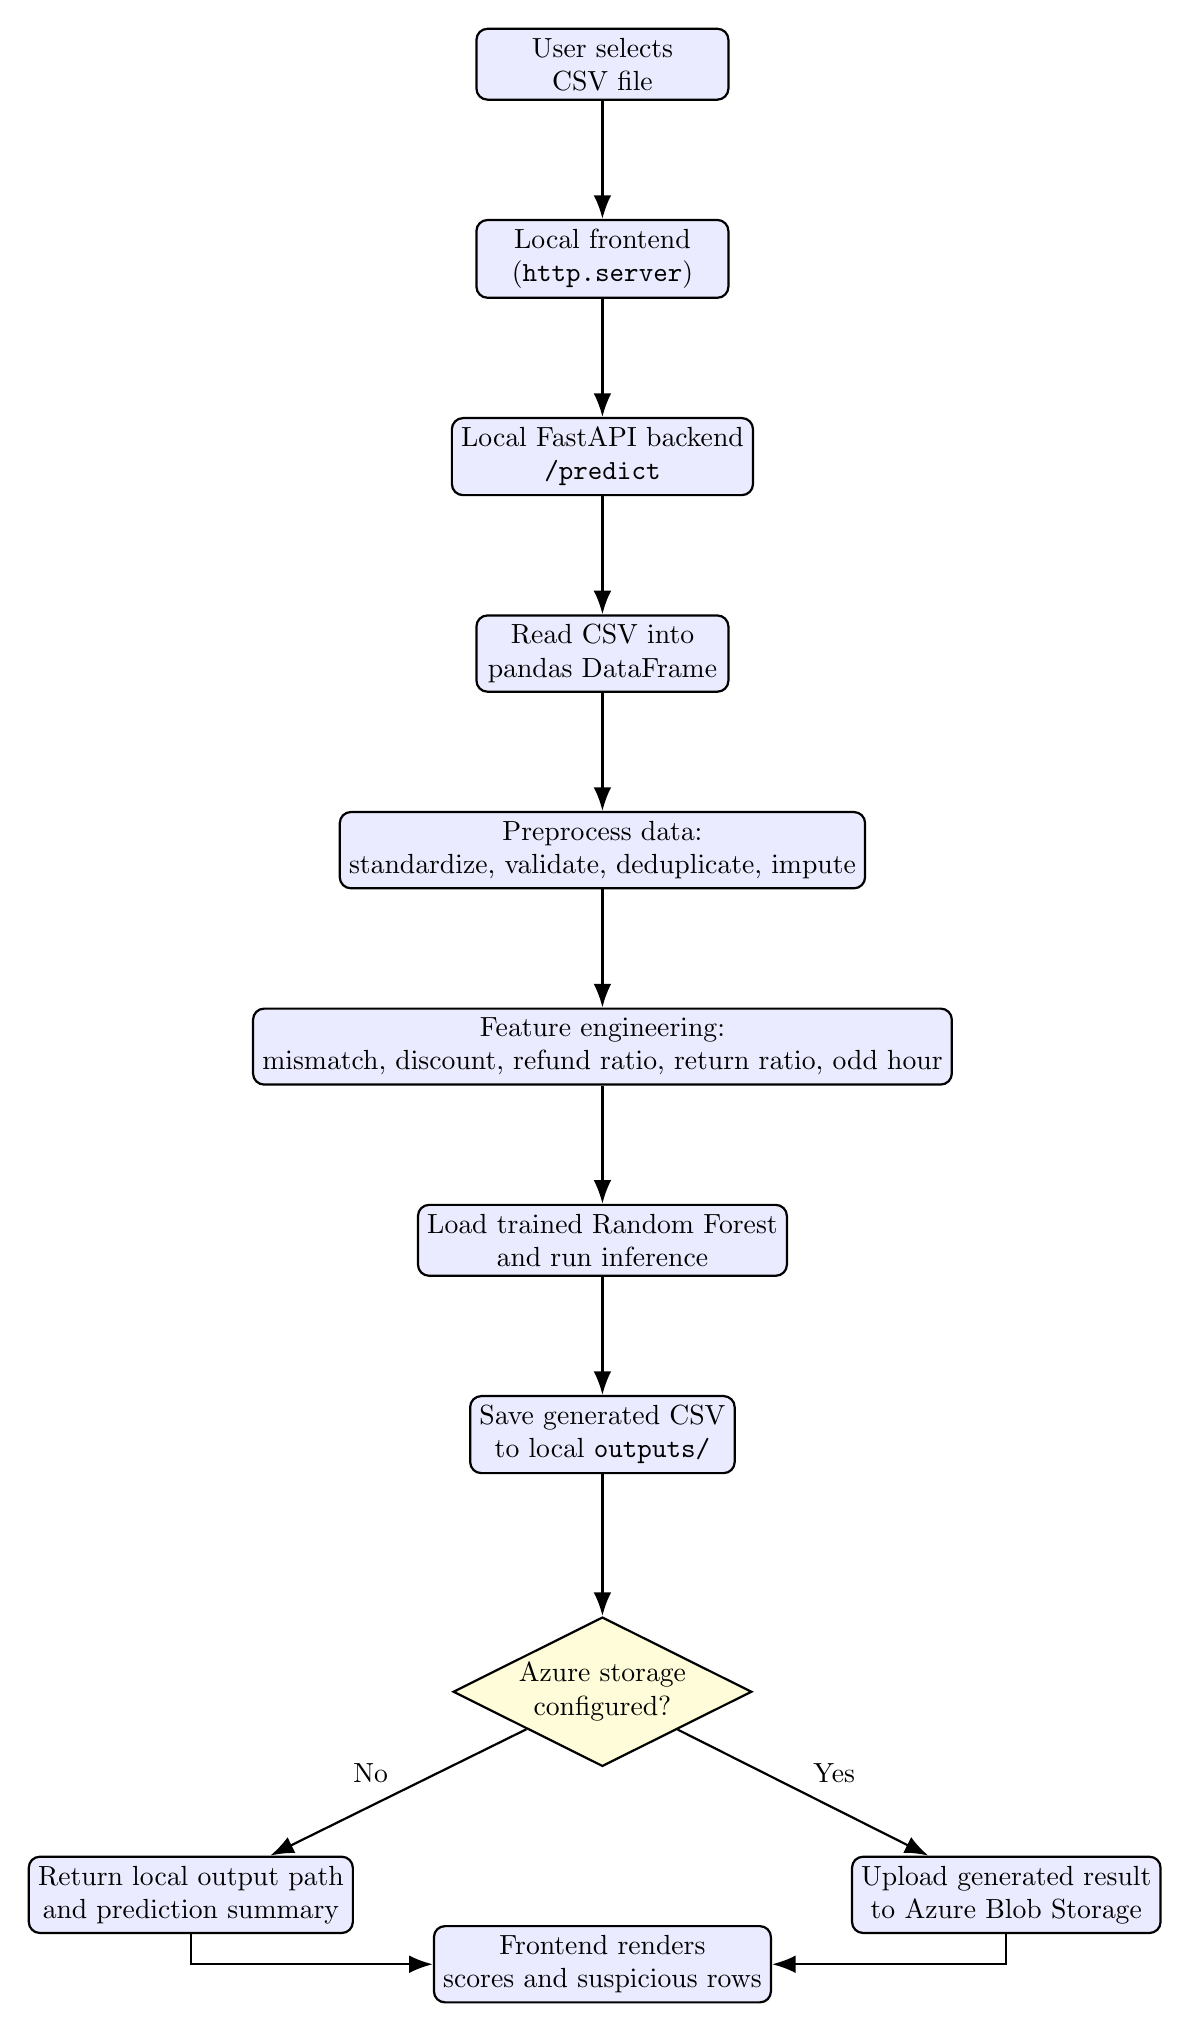
\begin{tikzpicture}[node distance=1.5cm]
\node[process] (user) {User selects\\CSV file};
\node[process, below=of user] (front) {Local frontend\\(\texttt{http.server})};
\node[process, below=of front] (api) {Local FastAPI backend\\\texttt{/predict}};
\node[process, below=of api] (read) {Read CSV into\\pandas DataFrame};
\node[process, below=of read] (prep) {Preprocess data:\\standardize, validate, deduplicate, impute};
\node[process, below=of prep] (feat) {Feature engineering:\\mismatch, discount, refund ratio, return ratio, odd hour};
\node[process, below=of feat] (model) {Load trained Random Forest\\and run inference};
\node[process, below=of model] (save) {Save generated CSV\\to local \texttt{outputs/}};
\node[decision, below=1.8cm of save] (decide) {Azure storage\\configured?};
\node[process, below left=1.6cm and 2.2cm of decide] (localreturn) {Return local output path\\and prediction summary};
\node[process, below right=1.6cm and 2.2cm of decide] (blob) {Upload generated result\\to Azure Blob Storage};
\node[process, below=2.0cm of decide] (render) {Frontend renders\\scores and suspicious rows};

\draw[arrow] (user) -- (front);
\draw[arrow] (front) -- (api);
\draw[arrow] (api) -- (read);
\draw[arrow] (read) -- (prep);
\draw[arrow] (prep) -- (feat);
\draw[arrow] (feat) -- (model);
\draw[arrow] (model) -- (save);
\draw[arrow] (save) -- (decide);
\draw[arrow] (decide) -- node[above left] {No} (localreturn);
\draw[arrow] (decide) -- node[above right] {Yes} (blob);
\draw[arrow] (localreturn) |- (render);
\draw[arrow] (blob) |- (render);
\end{tikzpicture}
\end{adjustbox}
\caption{Local machine execution flow of the project}
\end{figure}

\subsection{Flowchart for Azure Version}
\begin{figure}[htbp]
\centering
\begin{adjustbox}{max totalsize={\textwidth}{0.78\textheight},center}
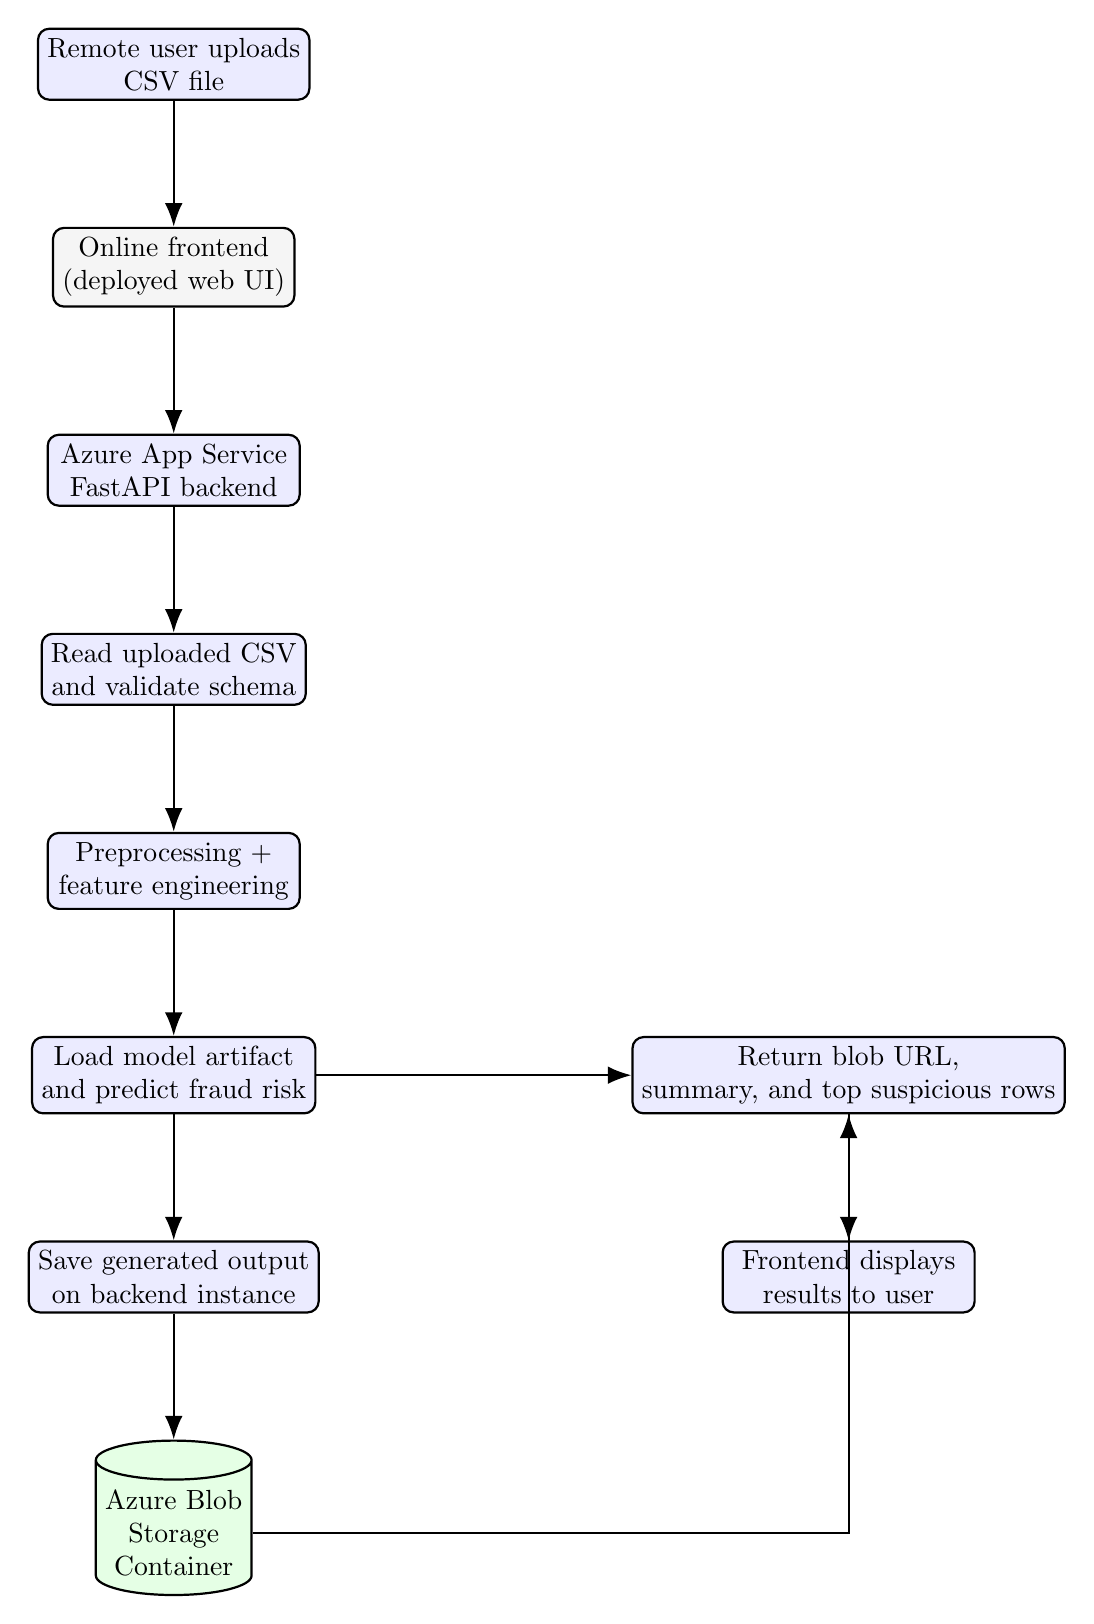
\begin{tikzpicture}[node distance=1.6cm]
\node[process] (remoteuser) {Remote user uploads\\CSV file};
\node[cloudbox, below=of remoteuser] (static) {Online frontend\\(deployed web UI)};
\node[process, below=of static] (appsvc) {Azure App Service\\FastAPI backend};
\node[process, below=of appsvc] (ingest) {Read uploaded CSV\\and validate schema};
\node[process, below=of ingest] (engg) {Preprocessing +\\feature engineering};
\node[process, below=of engg] (infer) {Load model artifact\\and predict fraud risk};
\node[process, below=of infer] (temp) {Save generated output\\on backend instance};
\node[store, below=of temp] (storage) {Azure Blob\\Storage\\Container};
\node[process, right=4.0cm of infer] (response) {Return blob URL,\\summary, and top suspicious rows};
\node[process, below=of response] (ui) {Frontend displays\\results to user};

\draw[arrow] (remoteuser) -- (static);
\draw[arrow] (static) -- (appsvc);
\draw[arrow] (appsvc) -- (ingest);
\draw[arrow] (ingest) -- (engg);
\draw[arrow] (engg) -- (infer);
\draw[arrow] (infer) -- (temp);
\draw[arrow] (temp) -- (storage);
\draw[arrow] (infer) -- (response);
\draw[arrow] (storage.east) -| (response.south);
\draw[arrow] (response) -- (ui);
\end{tikzpicture}
\end{adjustbox}
\caption{Azure-hosted execution flow of the project}
\end{figure}

\subsection{Azure-Based Architecture and Local Execution Diagram}
\begin{figure}[htbp]
\centering
\begin{adjustbox}{max totalsize={\textwidth}{0.82\textheight},center}
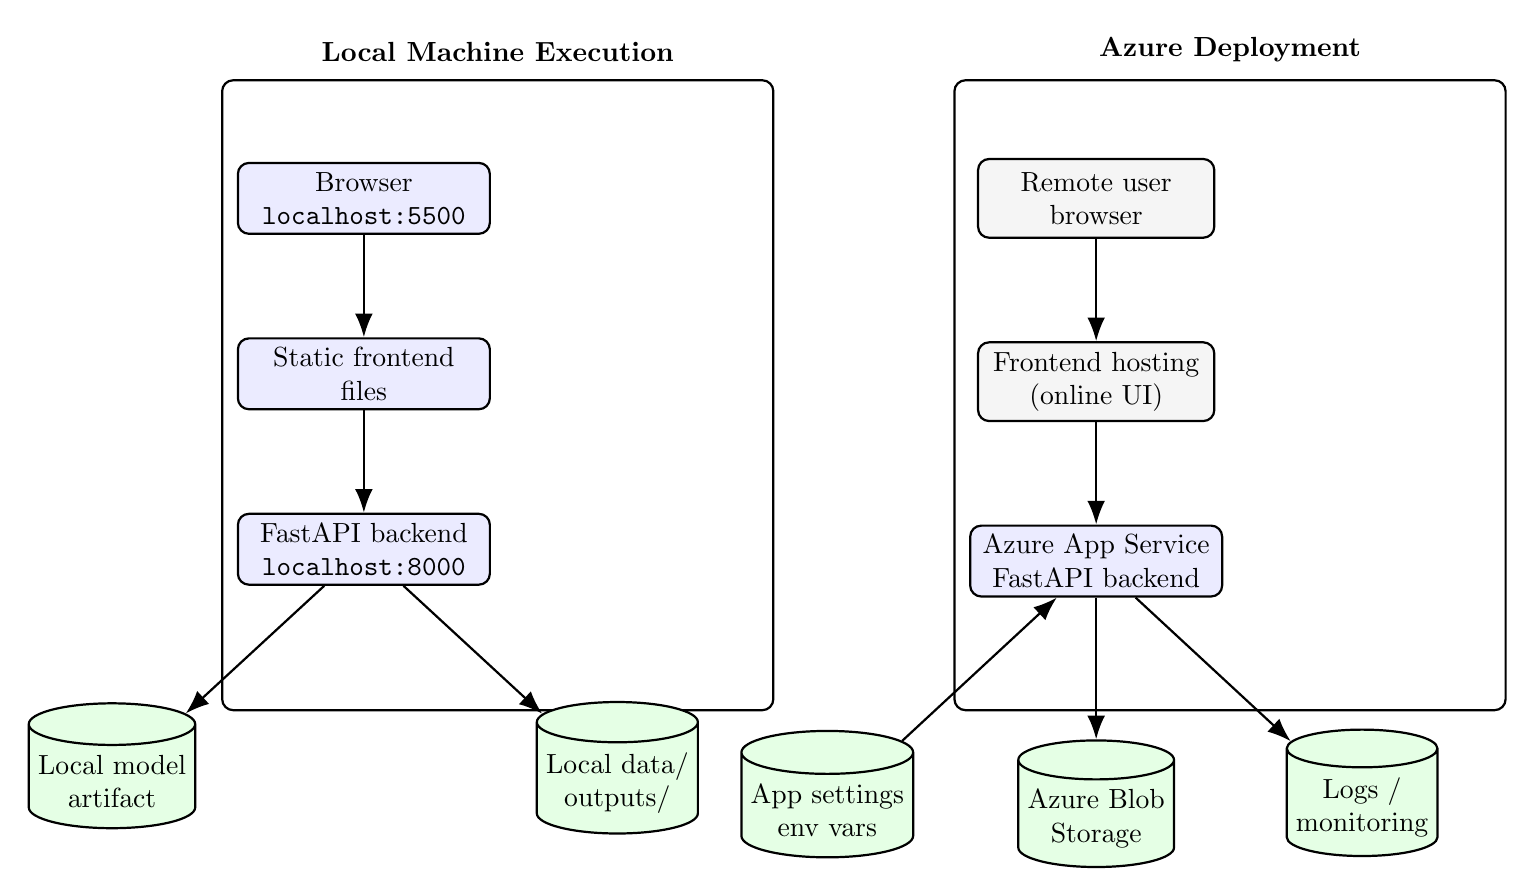
\begin{tikzpicture}[node distance=1.3cm]
\node[draw, thick, rounded corners, minimum width=7.0cm, minimum height=8.0cm, align=center] (localbox) at (0,0) {};
\node[above=0.1cm of localbox.north] {\textbf{Local Machine Execution}};
\node[process] (browserlocal) at (-1.7,2.5) {Browser\\\texttt{localhost:5500}};
\node[process, below=of browserlocal] (frontlocal) {Static frontend\\files};
\node[process, below=of frontlocal] (apilocal) {FastAPI backend\\\texttt{localhost:8000}};
\node[store, below left=1.6cm and 0.7cm of apilocal] (modellocal) {Local model\\artifact};
\node[store, below right=1.6cm and 0.7cm of apilocal] (fileslocal) {Local data/\\outputs/};
\draw[arrow] (browserlocal) -- (frontlocal);
\draw[arrow] (frontlocal) -- (apilocal);
\draw[arrow] (apilocal) -- (modellocal);
\draw[arrow] (apilocal) -- (fileslocal);

\node[draw, thick, rounded corners, minimum width=7.0cm, minimum height=8.0cm, align=center] (azurebox) at (9.3,0) {};
\node[above=0.1cm of azurebox.north] {\textbf{Azure Deployment}};
\node[cloudbox] (browsercloud) at (7.6,2.5) {Remote user\\browser};
\node[cloudbox, below=of browsercloud] (frontcloud) {Frontend hosting\\(online UI)};
\node[process, below=of frontcloud] (appcloud) {Azure App Service\\FastAPI backend};
\node[store, below left=1.8cm and 0.9cm of appcloud] (envcloud) {App settings\\env vars};
\node[store, below=1.8cm of appcloud] (blobcloud) {Azure Blob\\Storage};
\node[store, below right=1.8cm and 0.9cm of appcloud] (monitor) {Logs /\\monitoring};
\draw[arrow] (browsercloud) -- (frontcloud);
\draw[arrow] (frontcloud) -- (appcloud);
\draw[arrow] (envcloud) -- (appcloud);
\draw[arrow] (appcloud) -- (blobcloud);
\draw[arrow] (appcloud) -- (monitor);
\end{tikzpicture}
\end{adjustbox}
\caption{Comparison of local execution and Azure-based architecture}
\end{figure}
\FloatBarrier

\subsection{Module-Wise Explanation}
\begin{table}[H]
\centering
\caption{System Modules and Their Responsibilities}
\begin{tabular}{p{3cm} p{10.2cm}}
\toprule
\textbf{Module} & \textbf{Description} \\
\midrule
Data generation & Synthetic ERP-like dataset generation with fields such as order amount, quantity, discount, billing state, shipping state, account age, return history, refund amount, and fraud label. \\
Preprocessing & Standardizes column names, validates required columns, removes duplicate rows, converts numeric columns, and fills missing values using median and category defaults. \\
Feature engineering & Creates interpretable fraud indicators such as shipping mismatch flag, high discount flag, new customer high value flag, refund-to-order ratio, customer return ratio, urgent manual override flag, odd order hour flag, and high order amount flag. \\
Model training & Splits the data into training and testing sets and trains a Random Forest classifier with class balancing. \\
Prediction service & Loads the model artifact, computes \texttt{fraud\_risk\_score} and \texttt{suspicious\_flag}, and prepares a summary for the frontend. \\
Frontend & Provides a browser-based interface for entering the API URL, uploading CSV data, and viewing suspicious results. \\
Storage integration & Saves prediction results locally and uploads them to Azure Blob Storage when \texttt{AZURE\_STORAGE\_CONNECTION\_STRING} is configured. \\
Deployment layer & Supports localhost execution and Azure App Service deployment using the same underlying application logic. \\
\bottomrule
\end{tabular}
\end{table}

\subsection{Technical Basis of the Implemented Approach}
The current implementation uses a Random Forest classifier because tree-based ensemble methods perform well on structured tabular data and can capture nonlinear relationships without heavy feature scaling \cite{afriyie2023supervised,sulaiman2022review}. The project uses engineered business features rather than raw transaction fields alone, which improves interpretability and aligns with domain knowledge. In the Azure-hosted configuration, the backend uses App Service environment variables to obtain cloud configuration securely, while the frontend remains free of secrets. Generated prediction outputs are optionally uploaded to Blob Storage using the Azure Storage Python SDK \cite{azureappservice,azureblobpython}.

\section{Workdone So Far}
This section summarizes the modules completed to date and the observations obtained from the current implementation.

\subsection{Completed Modules}
\begin{enumerate}[noitemsep]
    \item Synthetic ERP transaction dataset generation.
    \item Raw data preprocessing and validation pipeline.
    \item Fraud-oriented feature engineering module.
    \item Baseline Random Forest model training and model artifact creation.
    \item FastAPI backend with \texttt{/health} and \texttt{/predict} endpoints.
    \item Browser-based frontend for CSV upload and results visualization.
    \item Local output generation in CSV format.
    \item Optional Azure Blob Storage upload for prediction output files.
\end{enumerate}

\subsection{Current Dataset and Model Snapshot}
\begin{table}[H]
\centering
\caption{Current Project Snapshot}
\begin{tabular}{p{5.5cm} p{5cm}}
\toprule
\textbf{Item} & \textbf{Current Value} \\
\midrule
Dataset size & 1000 rows \\
Fraud-positive rows & 97 \\
Training rows & 800 \\
Testing rows & 200 \\
Model type & Random Forest Classifier \\
Number of trees & 200 \\
Maximum tree depth & 10 \\
Saved model artifact & \texttt{models/fraud\_model.pkl} \\
Prediction output location & \texttt{outputs/} \\
Optional cloud output location & Azure Blob Storage container \texttt{outputs} \\
\bottomrule
\end{tabular}
\end{table}

\subsection{Observed Performance}
Evaluation of the currently trained baseline on the held-out test set produced the results shown in Table~\ref{tab:metrics}. These values were generated from the saved project model and dataset.

\begin{table}[H]
\centering
\caption{Baseline Model Performance}
\label{tab:metrics}
\begin{tabular}{p{5cm} p{3cm}}
\toprule
\textbf{Metric} & \textbf{Value} \\
\midrule
Accuracy & 0.9050 \\
Precision & 0.5000 \\
Recall & 0.0526 \\
F1-score & 0.0952 \\
ROC-AUC & 0.9331 \\
\bottomrule
\end{tabular}
\end{table}

\begin{table}[H]
\centering
\caption{Confusion Matrix of the Baseline Model}
\begin{tabular}{lcc}
\toprule
\textbf{Actual / Predicted} & \textbf{Legitimate} & \textbf{Fraud} \\
\midrule
Legitimate & 180 & 1 \\
Fraud & 18 & 1 \\
\bottomrule
\end{tabular}
\end{table}

\begin{figure}[H]
\centering
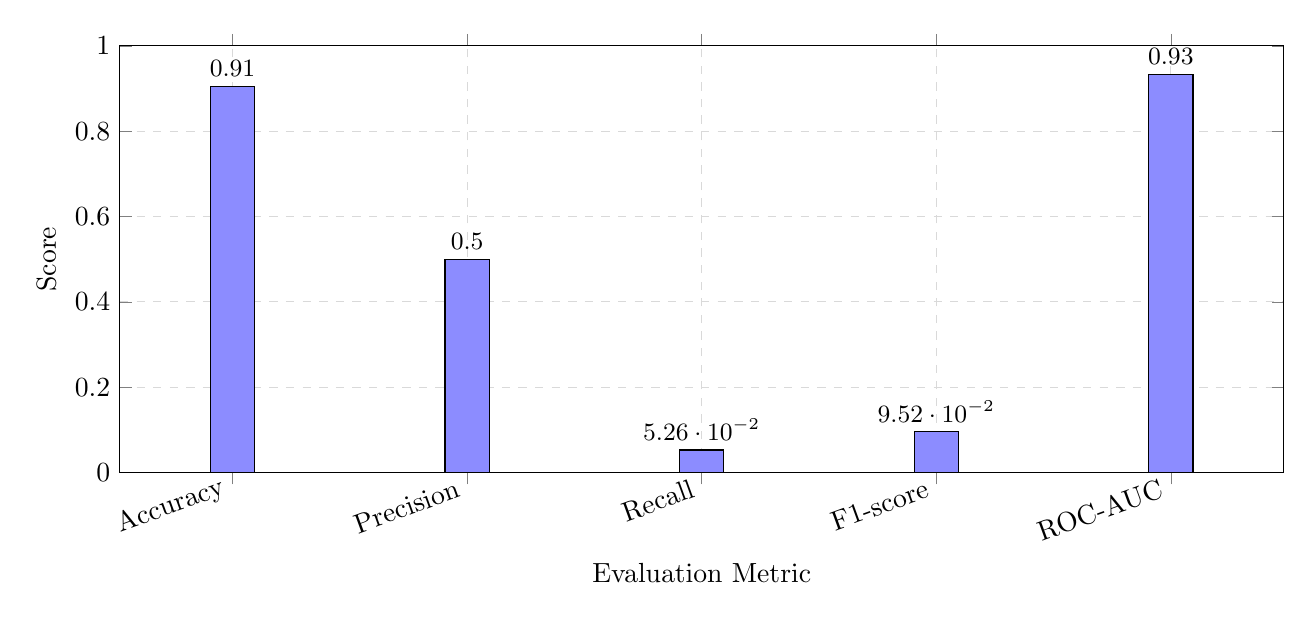
\begin{tikzpicture}
\begin{axis}[
    ybar,
    bar width=16pt,
    width=0.92\textwidth,
    height=7cm,
    ymin=0,
    ymax=1,
    symbolic x coords={Accuracy,Precision,Recall,F1-score,ROC-AUC},
    xtick=data,
    nodes near coords,
    nodes near coords align={vertical},
    ylabel={Score},
    xlabel={Evaluation Metric},
    enlarge x limits=0.12,
    grid=major,
    grid style={dashed,gray!30},
    every node near coord/.append style={font=\small},
    x tick label style={rotate=20, anchor=east}
]
\addplot[fill=blue!45] coordinates {
    (Accuracy,0.9050)
    (Precision,0.5000)
    (Recall,0.0526)
    (F1-score,0.0952)
    (ROC-AUC,0.9331)
};
\end{axis}
\end{tikzpicture}
\caption{Performance profile of the current baseline model}
\end{figure}

\subsection{Feature Importance Observations}
The current model indicates that the most influential predictors include shipping mismatch, refund-to-order ratio, customer return ratio, order amount, and account age. This is consistent with expected fraud behavior in transactional settings, where suspicious orders are often linked to unusual logistics and refund patterns.

\begin{figure}[H]
\centering
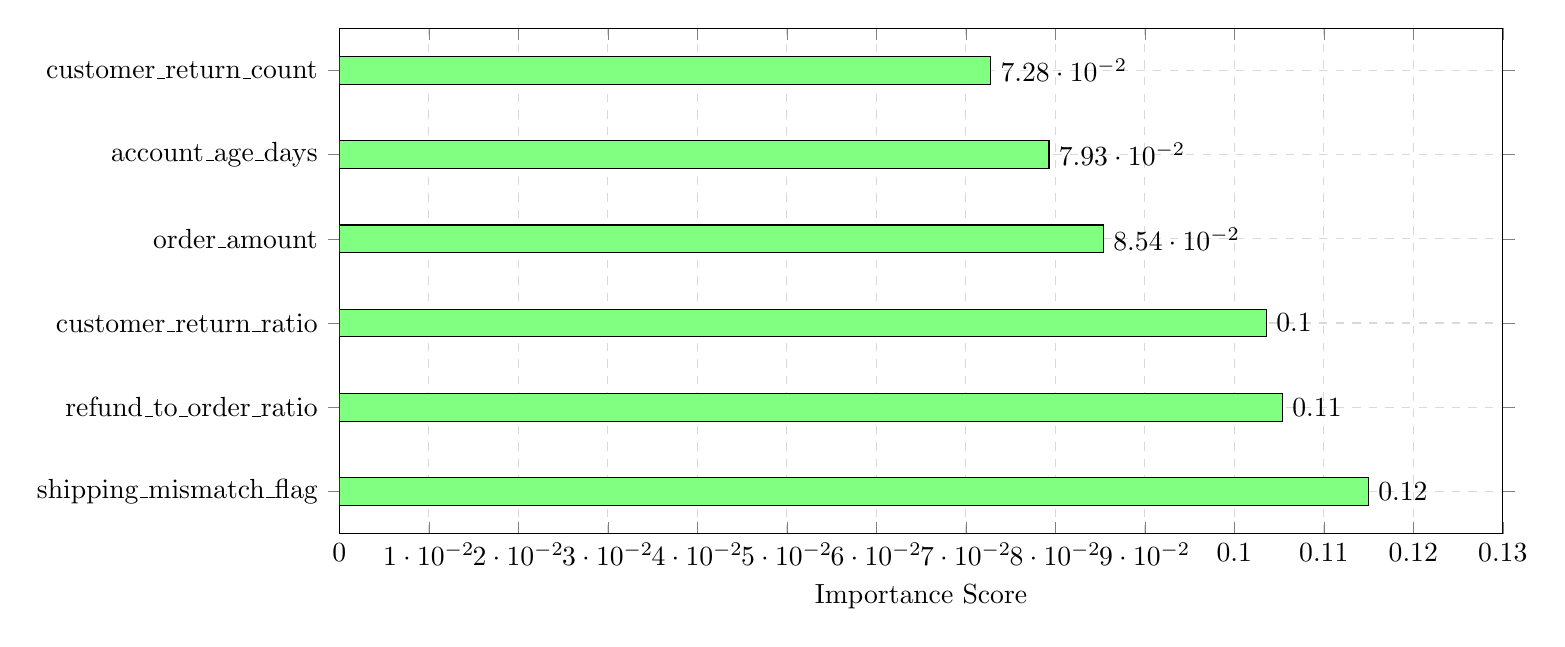
\begin{tikzpicture}
\begin{axis}[
    xbar,
    width=0.92\textwidth,
    height=8cm,
    xmin=0,
    xmax=0.13,
    xlabel={Importance Score},
    ytick=data,
    symbolic y coords={shipping\_mismatch\_flag,refund\_to\_order\_ratio,customer\_return\_ratio,order\_amount,account\_age\_days,customer\_return\_count},
    nodes near coords,
    nodes near coords align={horizontal},
    grid=major,
    grid style={dashed,gray!30}
]
\addplot[fill=green!50] coordinates {
    (0.1150,shipping\_mismatch\_flag)
    (0.1054,refund\_to\_order\_ratio)
    (0.1036,customer\_return\_ratio)
    (0.0854,order\_amount)
    (0.0793,account\_age\_days)
    (0.0728,customer\_return\_count)
};
\end{axis}
\end{tikzpicture}
\caption{Top feature importances from the current Random Forest model}
\end{figure}

\subsection{Functional Outcome of the Implemented System}
The current end-to-end prediction pipeline successfully processes uploaded transaction data and produces both row-level and summary outputs. On the available sample dataset, the system produced:
\begin{itemize}[noitemsep]
    \item \textbf{Total rows processed}: 1000
    \item \textbf{Suspicious rows flagged}: 80
    \item \textbf{Average suspicious risk score}: 0.7411
\end{itemize}

The results suggest that the model is able to rank risky records effectively, as indicated by the strong ROC-AUC value. However, the current operating threshold yields very low recall. This means the model is conservative and misses many true fraud cases. From a research perspective, this is a meaningful finding because it indicates that future work should focus on threshold tuning, class imbalance handling, and alternative models.

\section{Remaining Work}
Although the primary system pipeline is functional, several tasks remain before the research can be considered complete:
\begin{itemize}[noitemsep]
    \item Improve recall and F1-score through threshold tuning and model calibration.
    \item Evaluate imbalance-handling methods such as oversampling, undersampling, or cost-sensitive learning.
    \item Compare the baseline model with XGBoost, LightGBM, Isolation Forest, and Autoencoder-based alternatives.
    \item Perform cross-validation for more reliable performance estimation.
    \item Test the pipeline on more realistic or externally sourced ERP-like datasets.
    \item Improve the frontend by explicitly displaying the status of Azure Blob upload success or failure.
    \item Add stronger logging, monitoring, and operational error reporting.
    \item Harden the Azure deployment with better secret management and documentation.
\end{itemize}

\section{Scope}
The scope of this research extends beyond a classroom demonstration because the underlying problem is common across multiple industries. The proposed system can benefit:
\begin{itemize}[noitemsep]
    \item \textbf{Manufacturing and retail organizations}, which process large order volumes and require anomaly screening.
    \item \textbf{Supply chain management teams}, which need early identification of suspicious shipping and refund behavior.
    \item \textbf{ERP administrators and audit teams}, which can use fraud risk scores to prioritize manual review.
    \item \textbf{Academic researchers and students}, who can use this work as a reference for building explainable machine learning systems with cloud integration.
    \item \textbf{Small and medium enterprises}, which need low-cost fraud monitoring solutions that can run locally or in the cloud.
\end{itemize}

The project is especially valuable as a bridge between theoretical fraud detection research and practical system implementation.

\section{Future Work}
The present work establishes a baseline architecture and model. Future enhancements can make the system more accurate, scalable, and production ready:
\begin{itemize}[noitemsep]
    \item Introduce advanced classifiers such as XGBoost, CatBoost, and deep anomaly detection models.
    \item Add explainable AI techniques such as SHAP to justify why specific transactions are flagged.
    \item Move from batch CSV uploads to streaming or event-driven transaction scoring.
    \item Integrate Azure Application Insights for observability and performance tracing.
    \item Replace connection-string-based storage access with managed identity or Azure Key Vault.
    \item Support user authentication and role-based access for investigators and administrators.
    \item Extend the system to multi-class fraud categorization, such as refund abuse, discount abuse, and identity-risk orders.
    \item Expand the frontend into a richer dashboard with trend charts, download options, and case review workflow.
\end{itemize}

\section{Conclusion}
This progress report presents the design and implementation status of a machine learning-based fraud detection system for supply chain ERP transactions. The work completed so far demonstrates a functioning end-to-end pipeline that includes data preparation, fraud-oriented feature engineering, Random Forest-based inference, web API exposure, browser-based upload, and optional Azure Blob Storage integration. The current baseline achieves promising ranking performance but low recall, which provides a clear direction for the remaining research effort. Overall, the project forms a strong foundation for a practical and academically relevant fraud analytics system.

\newpage
\bibliographystyle{IEEEtran}
\bibliography{myref}

\end{document}
